%%%%%%%%%%%%%%%%%%%%%%%%%%%%%%%%%%%%%%%%%%%%%%%%%%%%%%%%%%%%%%%%%%%
%%% Documento LaTeX                                             %%%
%%%%%%%%%%%%%%%%%%%%%%%%%%%%%%%%%%%%%%%%%%%%%%%%%%%%%%%%%%%%%%%%%%%
% Título:   Apéndice A
% Autor:    Ignacio Moreno Doblas
% Fecha:    2014-02-01
% Versión:  0.5.0
%%%%%%%%%%%%%%%%%%%%%%%%%%%%%%%%%%%%%%%%%%%%%%%%%%%%%%%%%%%%%%%%%%%%

\pagestyle{fancy}
\fancyhead[LE,RO]{\thepage}
\fancyhead[RE]{Apéndice} %
\fancyhead[LO]{\nouppercase{\rightmark}}
%\fancyhead[RE]{Parte \thepart \rightmark} %

\chapterbegin{Funcionamiento de la macro ADDEXC}
\label{chp:MacroADDEXC}
\minitoc

\section{Finalidad y tipos de salto}

Queremos implementar una macro que nos permita codificar las
instrucciones de salto dentro del vector de interrupciones. Como en
la arquitectura el bus de direcciones es de 32 bits no podemos
codificar una instrucción de salto a cualquier dirección con
una instrucción de 32 bits, puesto que no nos queda espacio
para el código de operación.

Por esta razón existen dos tipos de salto, los saltos cortos
($\pm 32Mb$) y los saltos largos (todo el espacio de memoria). Un
salto corto (aplicable también a saltos condicionales) en
ensamblador se escribiría así.

\begin{lstlisting}
        b       etiqueta
\end{lstlisting}

Los saltos largos no tienen instrucción propia, se realizan mediante
la carga del registro {\tt pc} partiendo de un dato en memoria.

\begin{lstlisting}
        ldr     pc, a_etiq
        [...]
a_etiq: .word   etiqueta
\end{lstlisting}

Ésto en código máquina siempre se traduce a un direccionamiento
relativo a {\tt pc}, si estuviésemos depurando veríamos algo como
esto.

\begin{lstlisting}
        ldr     pc, [pc, #0x24]
\end{lstlisting}

Donde {\tt 0x24} es el desplazamiento (hemos elegido un valor arbitrario)
donde se encontraría {\tt a\_etiq}. De hecho esto mismo ocurre cuando utilizamos
{\tt ldr} con el operador {\tt =}, podríamos haber escrito esta otra instrucción
con idéntico resultado.

\begin{lstlisting}
        ldr     pc, =etiqueta
\end{lstlisting}

Es la forma de escribirlo en alto nivel, se produce exactamente el mismo código
máquina que en el caso anterior. Debemos recordar que las instrucciones donde
aparece el operador {\tt =} ocupan 8 bytes, 4 para la propia instrucción y otros
4 para el dato que generará de forma transparente el propio ensamblador.

\section{Elección: salto corto}

Si buscamos código por internet lo más normal es encontrar tablas de excepciones
completas que usan el salto largo en lugar del corto. Esto nos obliga a
rellenar una tabla en la que la mayor parte de vectores no se usan y a que
dicha tabla sea estática. Por esa razón nosotros emplearemos nuestro propio
método basado en el salto corto.

Una desventaja es que tenemos que traducir una dirección (la de la RTI) al
código máquina de un salto corto. Y la complicación viene más que nada porque
el salto corto es relativo, es decir, depende del valor que tenga {\tt pc} en
el momento del salto.

La otra desventaja es que no podemos saltar más allá de 32Mb, pero para esto tendríamos
que estar metidos en un proyecto bastante grande como para necesitar más de 32Mb
de código, y aún así podemos solventarlo ubicando las RTI al principio.

\section{Escribir una macro}

En la primera línea ponemos la directiva {\tt .macro} seguida del nombre de la macro
{\tt ADDEXC} y de los parámetros {\tt vector, dirRTI} separados por coma.

\begin{lstlisting}
      .macro    ADDEXC  vector, dirRTI
\end{lstlisting}

Luego escribiríamos el código de la macro, indicando los parámetros con
{\tt \textbackslash vector} y {\tt \textbackslash dirRTI} para acabar con {\tt .endm}.

\section{Codificación de la instrucción de salto}

Como las instrucciones son de 32 bits y siempre están alineadas a direcciones múltiplos
de 4, en lugar de codificar el desplazamiento en bytes se hace en número de
instrucciones (o grupos de 4 bytes). En código máquina una instrucción de salto
incondicional tiene el formato indicado en la figura \ref{fig:codsalto}.

\begin{figure}[h]
  \centering
    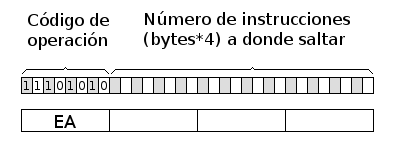
\includegraphics[width=14cm]{graphs/codsalto.png}
  \caption{Formato de instrucción de salto}
  \label{fig:codsalto}
\end{figure}

Los pasos para calcular la instrucción de salto serían.

\begin{itemize}
  \item Restar la dirección a saltar a la dirección actual
  \item Dividir entre 4
  \item Añadir {\tt 0xEA} al byte alto
\end{itemize}

Como todo son constantes en teoría podríamos implementar la
macro con dos instrucciones. Desgraciadamente el preprocesador
que usamos no es muy potente y si un operando es una etiqueta
sólo nos permite operar con sumas y restas. No podemos hacer las
divisiones o desplazamientos que necesitamos, con lo que emplearemos
una tercera instrucción para hacer el desplazamiento.

La dirección actual es {\tt \textbackslash vector}, la de la RTI
es {\tt \textbackslash dirRTI} y hay que restarle 8 por el
segmentado de la CPU.
\\
{\it instrucción }$ = (\textbackslash dirRTI-\textbackslash vector-8)/4 + 0xEA000000$ \\
{\it instrucción }$ = (\textbackslash dirRTI-\textbackslash vector)/4 + 0xE9FFFFFE$ \\
{\it instrucción }$ = (\textbackslash dirRTI-\textbackslash vector+3A7FFFFF8)/4$ \\
{\it instrucción }$ = (\textbackslash dirRTI-\textbackslash vector+A7FFFFFB) ror 2$

Vemos cómo en el último paso hemos transformado una división en una rotación, donde los
2 bits menos significativos (ambos a 1) pasan a ser los más significativos tras la
rotación.

\section{Resultado}

El código final queda como sigue.

\begin{lstlisting}
      .macro    ADDEXC  vector, dirRTI
        ldr     r1, =(\dirRTI-\vector+0xa7fffffb)
        ror     r1, #2
        str     r1, [r0, #\vector]
      .endm
\end{lstlisting}

Como la arquitectura no nos permite escribir en una dirección absoluta, antes
de invocar la macro debemos asegurarnos de que {\tt r0} apunte al vector de
interrupciones, es decir que valga {\tt 0}. En caso de usar esta macro como
primera instrucción del programa Bare Metal podemos omitir la inicialización
de {\tt r0}, ya que en las especificaciones de carga del {\tt kernel.img} se
establece este valor.

\chapterend
